\documentclass[xcolor ={table,usenames,dvipsnames}]{beamer}
\usepackage[italian]{babel}
\usepackage{color}
\usepackage{txfonts}
\PassOptionsToPackage{dvipsnames}{xcolor}
\title{Duck Typing in Python}
\author{Author: Tommaso Puccetti}
\institute{Universit\`a  degli Studi di Firenze}
\date{21/12/2018}
%\usepackage{sansmathaccent}
\usetheme{Berlin} 
\useinnertheme{rounded}
\useoutertheme{miniframes} 
\setbeamercovered{dynamic}
\theoremstyle{definition}
\newtheorem{definizione}{Definizione}
\usepackage{tikz}
\usetikzlibrary{arrows}
\usepackage{subfigure}

\begin{document}
	
	\begin{frame}
		\maketitle
			\begin{figure}[h!]
			\centering
			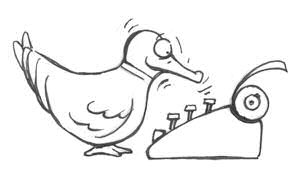
\includegraphics[scale=2]{img/cartoonduck.jpg}
			\label{Interfacce di un CS}
		\end{figure}
	\end{frame}

	\begin{frame}
		\frametitle{Introduction}
	\end{frame}
	
\end{document}